\documentclass[12pt,a4paper,titlepage]{article}
\usepackage[latin1]{inputenc}
\usepackage{amsmath}
\usepackage{amsfonts}
\usepackage{amssymb}
\usepackage{makeidx}
\usepackage{graphicx}
\usepackage{subcaption}

\makeatletter
\setlength{\@fptop}{0pt}
\makeatother

\oddsidemargin 1cm
\evensidemargin 1cm
\textwidth 15cm
\topmargin -1.25cm
\textheight 24.37cm

\renewcommand{\listfigurename}{Figures}
\renewcommand{\listtablename}{Tables}

\begin{document}	
	\begin{titlepage}
		\begin{figure}
			
\includegraphics[width=.6\linewidth]{images/logoWWU}
		\end{figure}
		\vspace*{2cm}
		\begin{center}
			Title:\\			
			\textbf{Application of Data Analytics in Failure Pattern Recognition}
			
			\vspace*{3cm}
			\textbf{Seminar Thesis}\\			
			In the context of the seminar ``Application of Data Analytics in Spare Parts Supply Chain Management''\\
			at the Chair for Information Systems and Supply Chain Management
		\end{center}
		\vspace*{1.5cm}
		\begin{tabbing}
			\hspace*{4cm}\= \kill
			Supervisors:			\> Dr.-Ing.Christian Grimme\\
									\> Dipl.-Inf. Jakob Bossek\\
									\> Carolin Wagner MScIS\\
			\\
			Presented by:			\> Alexander Anokhin\\
									\> Busso-Peus-Str. 14\\
									\> Muenster 48149\\
									\> Germany\\
									\> +4917675615943\\
									\> a\_anok01@uni-muenster.de\\
									\\
									\> Joshua Peter Handali\\
									\> Steinfurter Str. 81, Zi. 103\\
									\> Muenster 48149\\
									\> Germany\\
									\> +4915901002938\\
									\> j\_hand02@uni-muenster.de\\
			\\
			Date of submission: 	\> \today\\
		\end{tabbing}
	\end{titlepage}	
	
	\pagenumbering{gobble}
	\tableofcontents
	\newpage	
	
	\pagenumbering{Roman} 
	\setcounter{page}{1}
	\clearpage
	
	\addcontentsline{toc}{section}{Figures}
	\listoffigures
	\newpage
		
	\addcontentsline{toc}{section}{Tables}
	\listoftables
	\newpage
	
	\section*{Abbreviations}
	\addcontentsline{toc}{section}{Abbreviations}
	\begin{tabbing}
		\hspace*{5cm}\= \kill
		ANN				\> Artificial Neural Networks\\
		ANOVA RBF		\> ANOVA Radial Basis Function\\ 
		CART			\> Classification and Regression Trees\\
		CBM				\> Condition Based Maintenance\\
		CNN				\> Condensed Nearest Neighbour\\		
		DET				\> Distance Evaluation Technique\\
		ENN				\> Edited Nearest Neighbour\\		
		GA				\> Genetic Algorithm\\
		GS				\> Grid Search\\
		ICA				\> Independent Component Analysis\\
		NCL				\> Neighbourhood Cleaning Rule\\
		OSS				\> One-Sided Sampling\\
		PCA				\> Principal Component Analysis\\
		PSO			    \> Particle Swarm Optimization\\
		RFE				\> Recursive Feature Elimination\\
		SMOTE			\> Synthetic Minority Oversampling Technique\\
		SVM				\> Support Vector Machine\\		
	\end{tabbing}
	\newpage
	
	\pagenumbering{arabic} 
	\setcounter{page}{1}
	\section*{Introduction}
	\label{introduction}
	\addcontentsline{toc}{section}{Introduction}
	A successful failure pattern recognition system can go a long way in improving spare parts management in terms of allowing a good maintenance plan. Fault detection manifests itself as a part of condition based maintenance (CBM) \cite{McKee2014}. Failure pattern recognition maybe done not only to differentiate between failure and normal operation signals, but also to distinguish between different failure patterns. Identifying patterns benefits in early failure detection and investigation of root cause of failure. Meanwhile, distinguishing different failure patterns may lead to effective fault management action plans, as failures can then be accurately located. These opportunities lead to efforts on automatic failure pattern recognition, one of which can be done by applying classification algorithms such as Support Vector Machine (SVM).
	
	SVM is a relatively new computational learning method based on the statistical learning theory. Exhaustive overviews of SVM applicability in pattern recognition \cite{Lee2002} and fault diagnosis \cite{Widodo20072560} clearly show that SVM is a versatile and efficient technique for such problems. The concept of SVM is based on Vapnik-Chervonenkis theory \cite{cortes1995support, vapnik1995nature} that recently emerged as a general mathematical framework for estimating (learning) dependencies from finite samples \cite[p. 2561]{Widodo20072560}. The idea of SVM is to separate feature space by constructing linear boundary with the biggest margin between two classes. Moreover initial feature space can be enlarged with help of kernel transformations.
		
	SVM approach is not only theoretically well-founded, but also superior in practice. Recent surveys show that tuned SVM classifiers has become more efficient in pattern recognition than other methods: Artificial Neural Networks (ANN) \cite{Deng20116007, Jodas2013240, Kamruzzaman2006, pan2012parkinson, Shao201278} and Classification and Regression Trees (CART) \cite{marnerides2015fault, Shao201278}. In addition, SVMs have one significant advantage compared to conventional methods of pattern recognition such as ANNs. These methods straggle to solve problems with a small number of samples. For the reason that it is hard to obtain sufficient fault samples in practice, SVM is introduced into machines fault diagnosis due to its high accuracy and good generalization for a smaller number of samples \cite[p. 2562]{Widodo20072560}. 
	
	An aspect of pattern recognition task typically needs to be addressed is the class imbalance problem. It occurs where one or more classes heavily outnumber other classes. This is usually the case when putting patterns from normal operations and failure occurrences together, which also presents in datasets available for this paper. Comprehensive reviews on this matter are available in literatures \cite{Lopez2013113, Garcia2009} providing approaches to solve it. Sampling method is one of those approaches. It looks to train the classifier on a resampled dataset which involves reducing the size of majority classes and / or increasing the size of minority classes. Although sampling methods for binary classification tasks are more common, multi class sampling methods can also be found in researches \cite{multisampling, Yao2012}.
	
	Despite its robustness, SVMs are still susceptible to a degradation of performance when applied in imbalanced datasets \cite{Sun2009}. With that knowledge, basic sampling methods are pursued to explore their effects on this specific failure pattern recognition task using SVMs. Error rate are compared to investigate which sampling methods, if any, may improve the classification performance.  
	
	The first section of a paper describes underlying problem, research methodology and provided experimental data. Section 2 explores data preparation step which involves preprocessing the raw data and exploratory analysis. The analysis work starts with data balancing experiments in Section 3. This section covers both binary and multi class datasets. Section 4 provides a step-by-step SVM model building process, ranging from choice of kernel up to final model and further improvements. Additionally, dimensionality reduction and feature selection steps are also included in this section. Finally, Section 5 summarizes results of the analysis and outlines possibilities for future researches.   
	
	\section{Problem Description}
	\subsection{Research Methodology}
	Aim of analysis is to build a classifier, based on initially collected data, to detect failures. Such a diagnosis can highly benefit company in real life, since failures identified at early stage, future costly faults possibly prevented. The aim defines a number of research questions. First of all, it is unclear how the initially proposed data can be properly preprocessed. Moreover, since classes are possibly imbalanced another question is how they can be balanced and should they be balanced at all. Since feature extraction and selection as well as SVM parametrization are highly effect final results it will be also valuable to answer the question about optimal building procedure and parameters. Another question is how accuracy and efficiency of a classifier can vary along different settings, for example size of initial sample. 
	
	To accomplish the aim of a study research design is mainly based on optimization and simulation experiments, however literature research is also used in two ways: establishing a proper direction of analysis; identification of existing methods and approaches for further use. Analysis was conducted with help of R programming language\footnote{http://www.r-project.org/} which is used for statistical computing and graphics.
	
	\subsection{Data Description}
	The initial data is provided by a Brazilian manufacturer. The company produces different kinds of	electric actuators to drive control values. Data are generated in a test environment under normal and overload conditions. Three sensors are installed near the
	gears that are able to record the incurring vibration. The test environment is depicted at Figure \ref{fig:testEnvironment}. Sensor 1 is located in the bearing of the main spindle, Sensor 2 on the motor's bearing and Sensor 3 depicts a built-in torque sensor.
		
	\begin{figure}[h!]
		\centering
		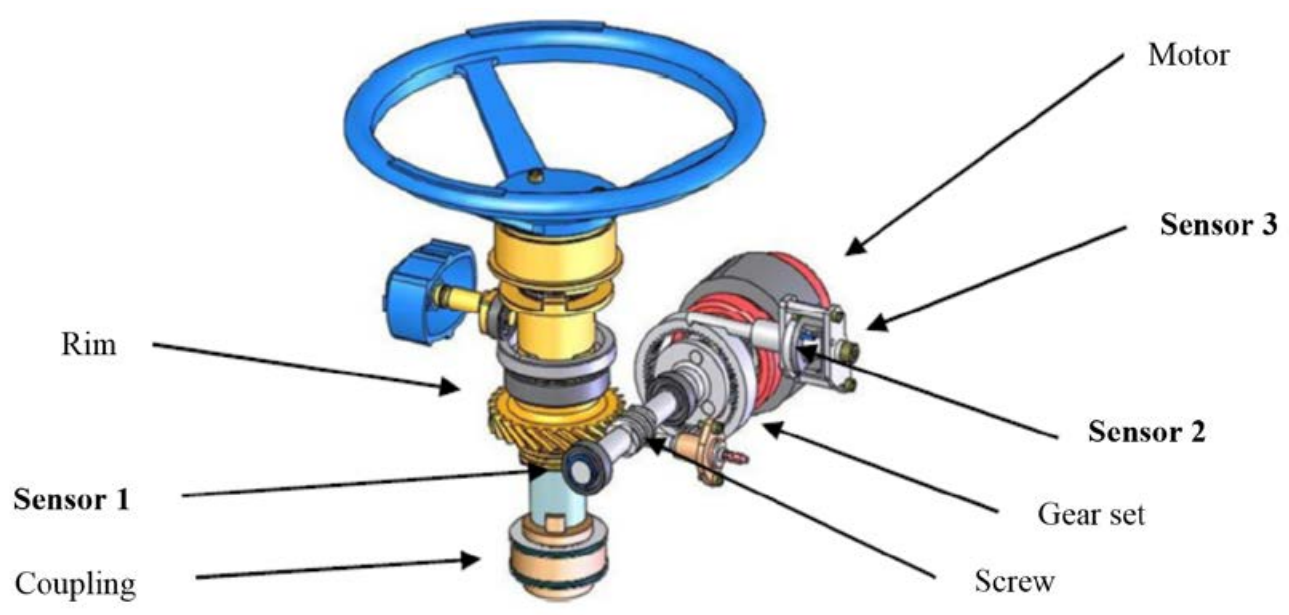
\includegraphics[width=1\linewidth]{images/testEnvironment}
		\caption{Test Environment}
		\label{fig:testEnvironment}
	\end{figure}	  
	
	Tests perform valve aperture actions and are initiated under different conditions. New gears are	considered with and without additional load. In addition, failure data is obtained using worn and broken gears therefore provided data comprises six different settings with three types of failures. For every second is collected 2048 observations of signal. Each cycle lasts about 46-47 seconds. Table \ref{table:generatedData} summarizes generated data.
	
	\begin{table}[h!]
		\centering
		\begin{tabular}{ | l | l | c | c | }
			\hline
			\multicolumn{1}{ | c | }{\textbf{Class}} 
				& \multicolumn{1}{ | c | }{\textbf{Description}}
				& \multicolumn{1}{ | c | }{\textbf{Cycles}} 	
				& \multicolumn{1}{ | c | }{\textbf{Observations}}\\
			\hline
			Normal 1 	& Cycle without load on actuator 			& 25 		& $2398*10^3$\\
			Normal 2 	& Cycle with pressure equal 3.0 bar 		& 25 		& $2572*10^3$\\
			Normal 3 	& Cycle with pressure equal 1.0 bar 		& 25 		& $2392*10^3$\\
			Failure 1 	& Cycle with a worn gear without load 		& 10 		& $930*10^3$\\
			Failure 2 	& Cycle with two worn gears without load 	& 2 		& $195*10^3$\\
			Failure 3 	& Cycle with a broken gear without load 	& 10 		& $946*10^3$\\
			\hline
		\end{tabular}
		\caption{Generated Data} 
		\label{table:generatedData}
	\end{table}
	
	Table \ref{table:generatedData} outlines three important aspects of further analysis. First, provided data are imbalanced along classes. The most unbalance case is between Normal 2 and Failure 2 classes. The unbalance ratio here accounts for 75:1000. Second, generated data consist of about 10 millions observations in total which makes computationally impossible to use SVM directly. Third, slightly more emphasis in analysis is putted on comparison of Normal 1 and failure classes since they have been all obtained without load. That is premised in assumption of being able to measure load directly. Since load is measured we can explicitly exclude classes with or without load depending on estimated load. 
	
	\section{Data Preparation}
	\subsection{Data Preprocessing}
	To achieve appropriate performance and classification results data preprocessing step should be done beforehand. The aim of data preprocessing from one side is to reduce the noise in the data and from another side retain as much information as possible. Typically data preprocessing also requires feature extraction step where a set of reasonable features extracted from raw signals.
	
	Generated data contain no missing data or obvious outliers which makes preprocessing step very straightforward. However one issue that affected performance at early stages is discovered. Every cycle has steady states in the beginning and in the end where signal does not change over about one second. That obviously distracts classifier since steady signal can be misclassified as failure which lead to full stop. To avoid such scenarios every second in a cycle is divided into 16 time windows and then for all of them standard deviation is calculated. In result if standard deviation is less than 5\% quantile for a whole cycle then signal during that period of time is considered as stable and related observations removed from further consideration. Figure \ref{fig:signalBehavior} shows this procedure. 
	
	\begin{figure}[h!]
		\centering
		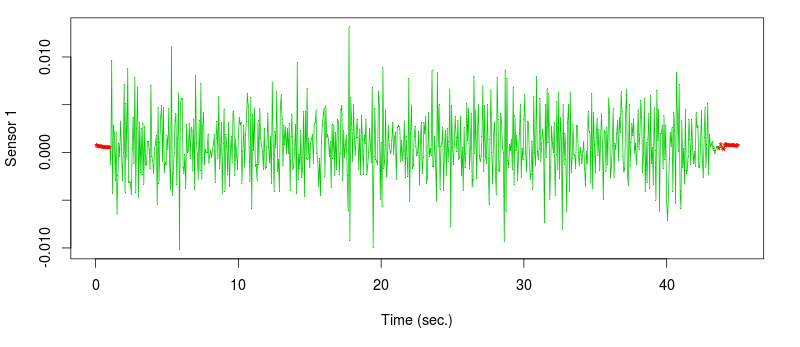
\includegraphics[width=1\linewidth]{images/signalBehavior}
		\caption[Signal Behavior]{Signal Behavior. Red line represents removed observations.}
		\label{fig:signalBehavior}
	\end{figure} 	
		
	Feature extraction step for vibration signal has been already widely explored in literature. Samanta \cite{Samanta2004625} during this step extracted time domain features in order to identify gear faults. That approach was later improved by Soleimani et al. \cite{soleimani2009fault}, vibration was considered not just as time varying but also as a physical signal, thus time domain and frequency domain features were extracted. In this analysis, based on existing research conducted by Soleimani et al. \cite[p. 2]{soleimani2009fault}, vibration signal is considered in time interval of 5 seconds where time domain features are extracted. Table \ref{table:extractedFeatures} presents extracted time domain features.
	
	\begin{table}[h!]
		\centering
		\begin{tabular}{ | l | l | }
			\hline
			\multicolumn{1}{ | c | }{\textbf{Feature}} 
				& \multicolumn{1}{ | c | }{\textbf{Formula}}\\
			\hline
			mean 				& $T_1=\frac{1}{N}\sum_{i=1}^{N}x_i$\\
			standard deviation 	& $T_2=(\frac{1}{N}\sum_{i=1}^{N}(x_i-T_1)^2)^{0.5}$\\
			peak 				& $T_3=max\{x_i\}, i=1,...,N$\\
			root mean square 	& $T_4=(\frac{1}{N}\sum_{i=1}^{N}x_{i}^{2})^{0.5}$\\
			crest factor 		& $T_4=\frac{T_3}{T_4}$\\
			skewness 			& $T_4=\frac{1}{T_{2}^{6}}\sum_{i=1}^{N}(x_{i}-T_1)^3$\\
			kurtosis 			& $T_4=\frac{1}{T_{2}^{8}}\sum_{i=1}^{N}(x_{i}-T_1)^4$\\
			\hline
		\end{tabular}
		\caption{Extracted Time Domain Features} 
		\label{table:extractedFeatures}
	\end{table}	
	
	After data preprocessing and feature extraction size of data was significantly reduced even without feature selection step. Final training sample consist of about 920 observations in total that makes possible to apply SVM in order to classify gear failures. Every observation  consists of 21 features: 7 extracted features for every sensor signal, and  response variable which shows existence of failure.
	
	\subsection{Exploratory Analysis}
	\label{exploratoryAnalysis}
	Another important step in order to build classifier is exploratory analysis. The aim of exploratory analysis is to understand data and check possible underlying assumptions required for analysis. It helps to find incentives for further steps and omit impossible scenarios which saves time and resources. SVM approach is very versatile and does nor require data to follow specific distribution that fact shortened exploratory step. 
	
	Since features are extracted from one signal there is a possibility that some of them are highly correlated and will create unnecessary computational overhead, during the process of training, without improvement of accuracy. It can be clearly seen from Table \ref{table:correlationMatricesOne} that features correlate along one sensor, for example, standard deviation of signal from Sensor 1 functionally determines root mean square for the same signal. In addition, features from different sensors correlate as well. Standard deviation of signal from Sensor 2 correlates with standard deviation of signal but from Sensor 3, which is shown at Table \ref{table:correlationMatricesAll}. These issues highlights the problem of dimensionality reduction which will be explored further in Section \ref{dimensionalityReduction}. 
	
	\begin{table}[h!]
		\begin{subtable}{.5\linewidth}
			\centering
			\begin{tabular}{ p{.4cm} | p{.4cm} | p{.4cm} | p{.4cm} | p{.4cm} | }
				  			& \textbf{1} 	& \textbf{2} 	& \textbf{3} 	& \textbf{4}\\ \hline
				\textbf{1} 	& 1 			& 0 			& .04 			& 0\\ \hline
				\textbf{2} 	&  				& 1 			& .57 			& 1\\ \hline
				\textbf{3} 	&   			&   			& 1 			& .57\\ \hline
				\textbf{4} 	&   			&   			&   			& 1\\ \hline
			\end{tabular}
			\caption{Sensor 1}
			\label{table:correlationMatricesOne}
		\end{subtable}
		\begin{subtable}{.5\linewidth}
			\centering
			\begin{tabular}{ p{.4cm} | p{.4cm} | p{.4cm} | p{.4cm} | }
				  			& \textbf{5}	& \textbf{6} 	& \textbf{7}\\ \hline
				\textbf{5} 	& 1				& .02 			& .4\\ \hline
				\textbf{6} 	&   			& 1 			& .54\\ \hline
				\textbf{7} 	&   			&   			& 1\\ \hline
			\end{tabular}
			\caption{All Sensors}
			\label{table:correlationMatricesAll}
		\end{subtable}
		\caption[Correlation Matrices]{Correlation Matrices. 1 - mean; 2 - standard deviation; 3 - peak; 4 - root mean square; 5, 6, 7 - standard deviations for sensors 1, 2, 3 respectively.}		
	\end{table}
		
	It was outlined before that SVM approach tries to find distinguishing hyperplane between two classes therefore during exploratory analysis it is also valuable to explore how separable observations from different classes. Figure \ref{fig:visualInspection} shows that some classes can be accurately separated using only two features. However it is not the common case for two-dimensional space where some classes have a lot of overlap. For example, classes with normal conditions are hardly separable in two-dimensional space. Of course, using more than two features can lead to accurate separation but it cannot be properly visualize. 
	
	\begin{figure}[!h]
		\begin{subfigure}{.5\textwidth}
			\centering
			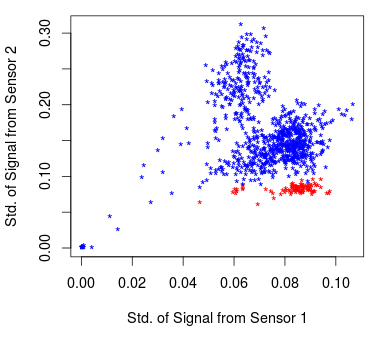
\includegraphics[width=.8\linewidth]{images/visualInspection1}
			\caption{Failure 1}
		\end{subfigure}%
		\begin{subfigure}{.5\textwidth}
			\centering
			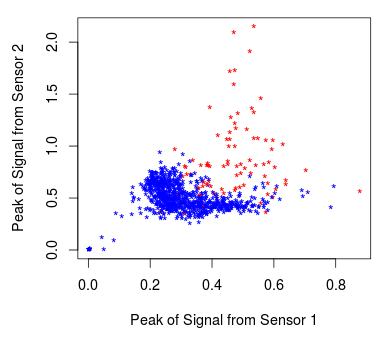
\includegraphics[width=.8\linewidth]{images/visualInspection2}
			\caption{Failure 3}
		\end{subfigure}
			\caption[Separation of Classes]{Separation of Classes. Red stars represent certain failure classes, blue points represent the rest of observations.}
		\label{fig:visualInspection}
	\end{figure}	
	
	Exploratory part here does not pretend to be exhaustive but the main goal is satisfied. Namely it helped understand more deeply data and provided further incentives: extracted features are correlated; separation of classes is possible however there is overlap between some classes.    
		
	\section{Data Balancing}	
	\subsection{Sampling Methods}
	\label{samplingMethods}
	There are eight different sampling methods plus a variant of one of those methods for the binary experiment. The original articles for each algorithms are cited accordingly, although this paper used their implementations available in the \textit{unbalanced}\footnote{https://cran.r-project.org/web/packages/unbalanced/unbalanced.pdf} package on R. The algorithm multi class sampling method, however, is directly implemented according to its source article while still utilizing a couple basic sampling algorithms from the previously mentioned R package.
	\\\\
	\textbf{Binary Sampling Methods}
	\begin{description}
	\item[Random Oversampling (ros)]
	Random replication of minority instances until the minority class is inflated to the size of majority class.
	
	\item[Random Undersampling (rus)]
	Random removal of majority instances until the majority class is reduced to the size of minority class.
	
	\item[Condensed Nearest Neighbour (cnn)]
	Hart's condensed nearest neighbour (CNN) rule \cite{cnn} selects a subset of majority instances. This subset needs to correctly classify instances of the original majority class using the 1-nearest neighbour rule.
	
	\item[Edited Nearest Neighbour (enn)]
	Wilson's edited nearest neighbour (ENN) rule \cite{enn} removes majority instances that differ from the majority of its 3-nearest neighbours.
	
	\item[One-Sided Sampling (oss)]
	One-Sided Sampling (OSS) \cite{oss} is a combination of CNN and Tomek links. A majority class subset is created by using CNN. Majority instances in this subset which participates in Tomek links are removed.
	
	\item[Neighbourhood Cleaning Rule (ncl)]
	Neighbourhood cleaning rule (NCL) \cite{ncl} applies an ENN variant and removes two subsets of majority instances. Firstly, Majority instances misclassified by their 3-nearest neighbours are removed. Secondly, it removes majority instances belonging to the 3-nearest-neighbours of minority instances.
	
	\item[Tomek link (tom)]
	Tomek links \cite{tomek} are pairs of different classed instances which are also each other's nearest neighbour. Majority instances which are Tomek links are removed.
	
	\item[Synthetic Minority Oversampling Technique (smoD and smo50)]
	Synthetic Minority Oversampling Technique (SMOTE) \cite{smote} creates new minority instances by interpolating feature values between minority instances and one or more of its 5 minority class nearest neighbours. This oversampling procedure through SMOTE is followed by undersampling the majority class. The resampling procedure is done by randomly sample with replacement a certain number of majority instances to be included into the new training set. Consequently, there are parameters which indicate the oversampling and undersampling rates. The default values are 200\% for both resampling rates. It means two new minority instances are generated for every original minority instances and two majority instances are randomly included into the resampled training set for every new minority instances. A simple tweak to oversampling rate leads to two different variants implemented in this paper.
	
	The first variant (smoD) is the one with default rates, which makes the minority class three times its original size and the majority class 1.33 times of the new minority class size. Note that because the undersampling rate doesn't take into account the original majority class' size, it may inflate the majority class size. This occurs when the size of majority class is smaller than four times the size of minority class, which was the case for some of the binary datasets being worked on.
	
	The second variant (smo50) is set up with two purposes, to create a 50:50 class ratio and to avoid increasing the size of majority class. Hence, the oversampling rate is set to 100\%, while the undersampling rate is left at 200\%, as the majority to minority ratio in the binary datasets are all larger than 2:1.
	\end{description}
	
	\begin{description}
	\item[Multi Class Sampling Methods]
	Two fairly straightforward methods to balance out sizes of multiple classes in one dataset are adapted from \cite{multisampling}, namely Standard Mean (SMean) and Standard Median (SMedian). Both methods create a multi class dataset with equal class sizes. In order to decide this final class size SMean takes the arithmetic mean of all class sizes, while SMedian takes the median class size of those classes. If a class is larger than the final class size it would be randomly undersampled, otherwise random oversampling is applied to that class.
	\end{description}
			
	\subsection{Experimental Setups}
	All experiments in this section utilize a non-optimized SVM classifier with the Radial Basis Kernel. Furthermore, a 20-fold cross validation is performed on the training data to provide an evaluation measure which is the cross validation error rate.
	
	\begin{description}
	\item[Binary Datasets]
	A total of nine binary datasets are included in this initial resampling implementation experiment. Each dataset is a combination of one of the three failure types and one of the three normal types. The number of majority and minority instances along with the majority to minority ratio for each dataset are presented in Table \ref{table:binaryratio}. All nine binary sampling methods described in the previous subsections are applied to these datasets. Furthermore, every method and dataset combination is repeated ten times, yielding 90 cross validation error rates for each sampling method.

\begin{table}[h!]
		\centering
		\begin{tabular}{ l | l | l | l |}
			\multicolumn{1}{ c | }{\textbf{}}
				& \multicolumn{1}{ | c | }{\textbf{Fail. 1}} 
				& \multicolumn{1}{ | c | }{\centering \textbf{Fail. 2}}
				& \multicolumn{1}{ | c | }{\centering \textbf{Fail. 3}}\\
			\hline
			\textbf{Norm. 1} & 2.6:1 				& 2.8:1 			& 2.6:1\\			
			\textbf{Norm. 2} & 12.3:1 				& 13.7:1 		& 12.1:1\\			
			\textbf{Norm. 3} & 2.6:1 				& 2.8:1 			& 2.6:1\\				
			\hline
		\end{tabular}
		\caption[Class Ratios of the Binary Datasets]{Class ratios of the binary datasets (Normal:Failure)} 
		\label{table:binaryratio}
	\end{table}	

\item[Multi Class Dataset]
Three failure types and three normal types are all put together into a unified dataset. This 6-class dataset is then subjected to four different training setups: one is directly using the dataset for training and the other three are balancing techniques. These balancing techniques are the two multi-class sampling methods, SMean and SMedian with random over- and under-sampling, and a simple class weighting scheme. Equation \ref{eq:weight} describes this weighting scheme, where $c_{i}$ and $n_{i}$ are the weight and size of class $i$ respectively and $k$ is the number of classes. The weights are normalized so that they all sum up to one. Each of these four SVM training setups is repeated a hundred times. One hundred cross validation error rates for every setups are used for comparison.

	\begin{equation} \label{eq:weight}
	c_{i} = \frac{\sum_{i=1}^{k=6} n_{i}}{n_{i}} * (\sum_{i=1}^{k=6} \frac{\sum_{i=1}^{k=6} n_{i}}{n_{i}})^{-1}
	\end{equation}

\end{description}
		
		\subsection{Experimental Result Analysis}		
	Both experiments are analyzed with the same approach. It involves visual inspection of each sampling method's cross validation error rates distributions through boxplot visualization and 	statistical tests to compare the methods performance with each other. The Friedman test and post-hoc Nemenyi test are employed as suggested by \cite{compare}. These statistical tests are intended to tell if there are any significance difference between how each method ranks within the same iteration, and across nine different datasets in the binary problem. Boxplots for the binary and multi class experiments are shown in Figure \ref{fig:binarybox} and Figure \ref{fig:multibox} respectively. As Friedman tests on both experiment indicate statistical significance, important parts of the post-hoc Nemenyi tests are presented in Table \ref{table:binarytest} and Table \ref{table:multitest} for the binary and multi class experiments respectively.
	
		\begin{figure}[h!]
			\centering
			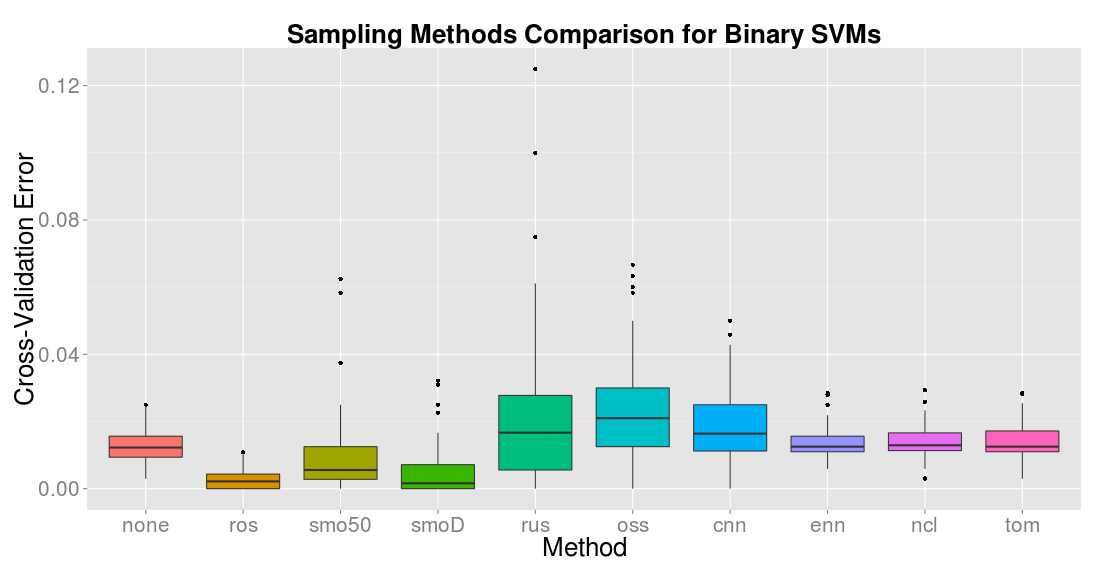
\includegraphics[width=1\linewidth]{images/binarybox}
			\caption[Sampling Methods for Binary SVMs]{Sampling Methods for Binary SVMs. Each boxplot contains 90 observations, 10 observations for each binary datasets.}
			\label{fig:binarybox}
		\end{figure}
		
		\begin{figure}[h!]
			\centering
			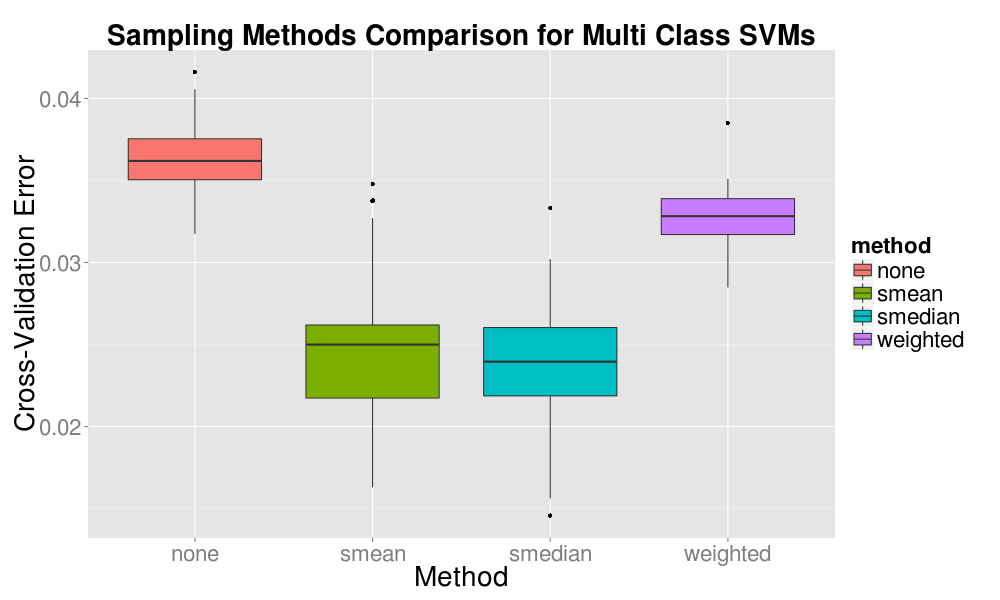
\includegraphics[width=1\linewidth]{images/multibox}
			\caption[Sampling Methods for Multi Class SVMs]{Sampling Methods for Multi Class SVMs. Each boxplot contains observations from 100 repeated runs on the 6-class dataset to train the SVM using the respective balancing method.}
			\label{fig:multibox}
		\end{figure}
		
		\begin{table}[h!]
		\centering
		\begin{tabular}{ | l | l | }
			\hline
			\multicolumn{1}{ | c | }{\textbf{Method}} 
				& \multicolumn{1}{ | c | }{\textbf{$p$-value}}\\
			\hline
			Random Oversampling (ros) 				& $1.4*10^{-12}$\\
			SMOTE with 100\% Oversampling Rate (smo50) 	& 0.009\\
			SMOTE with 200\% Oversampling Rate (smoD) 				& $6.6*10^{-11}$\\
			Random Undersampling (rus) 	& 0.318\\
			One-Sided Sampling (oss) 		& $3.3*10^{-5}$\\
			Condensed Nearest Neighbour (cnn) 			& 0.048\\
			Edited Nearest Neighbour (enn)			& 0.999\\
			Neighbourhood Cleaning Rule (ncl) 			& 0.594\\
			Tomek link (tom) 			& 0.697\\
			\hline
		\end{tabular}
		\caption[Statistical Significance of Sampling Methods for Binary Datasets]{Reported p-value from Nemenyi test for the performances of nine sampling methods compared to training on the original binary datasets.} 
		\label{table:binarytest}
	\end{table}	
		
		\begin{table}[h!]
			\centering
			\begin{tabular}{ | l | l | l | l |}
					\hline
					  			& \textbf{none} 	& \textbf{smean} 	& \textbf{smedian}\\ \hline
					\textbf{smean} 	& $< 2*10^{-16}$ & -	& -\\ \hline
					\textbf{smedian} 	& $< 2*10^{-16}$ & 0.96 & -\\ \hline
					\textbf{weighted} 	& $	1.9*10^{-7}$ & $2.7*10^{-13}$ & $5.7*10^{-14}$\\ \hline
				\end{tabular}
			\caption{Reported p-value from Nemenyi test for the performances of three balancing methods compared to training on the original multi class dataset (none).} 
			\label{table:multitest}
		\end{table}
		
	\begin{description}
	\item[Binary Datasets] Table \ref{table:binarytest} suggests that all three oversampling based methods, the random oversampling and two SMOTE variants, performed significantly better that training without data balancing. However, Figure \ref{fig:binarybox} provides further insight about the cross validation error rate distributions between those three sampling methods. Both random oversampling and the default SMOTE implementation (smoD) seem to have minimal overlap with training results on imbalanced datasets. Furthermore, the SMOTE variant which enforces majority class shrinkage (smo50) appears to vary more. A suggested cause here is that in 'smoD' there are cases where the majority class are actually randomly oversampled instead of undersampled, potentially avoiding information loss from the undersampling step of SMOTE. The major take-away here is that in this particular case of data imbalance inflating the size of minority classes, which are the failure patterns, may lead to significance improvement of SVM performance in terms of having low error rate. Undersampling, however, seems to cause important information loss of normal patterns.   
	\item[Multi Class Dataset] Taking a look at Table \ref{table:multitest}, all four scenarios appear to be significantly different except when comparing the two sampling methods SMean and SMedian. Moreover, by consulting Figure \ref{fig:multibox}, all three data balancing approaches produced improved performances with sampling methods out performing the naive weighting scheme. As a definite sampling method is needed for the next section, a rather conservative choice of using SMean is taken. While both methods performed practically the same in terms of error rate, SMean provides a slightly smaller class size of 153 instances compared to SMedian's 160 and maintains roughly the same dataset size to that of the original's.
	\end{description}

	
	\section{SVM Classifier}
	\subsection{Choice of Kernel}
	Kernels make SVM able to map initial feature space into high dimensional one and find there decision boundary without additional computational overhead. Appropriate choice of such a transformation highly influence accuracy of classifier. It is open question in almost any research in area of failure pattern recognition. There is no general rule for choosing a specific kernel. However in recent years there is a tendency to use Radial Basis Kernel as a benchmark.
	
	In order to estimate the optimal transformation standard SVM classifiers are build on balanced training data with different kernels: Linear, Polynomial, Radial Basis, Laplacian and ANOVA Radial Basis Function (ANOVA RBF). Each kernel transformation was used with default parameters specified in function \textit{ksvm} of package \textit{kernlab}\footnote{https://cran.r-project.org/web/packages/kernlab/kernlab.pdf} built in R. 
	
	\begin{table}[h!]
		\centering
		\begin{tabular}{ | l | c | c | }
			\hline
			\multicolumn{1}{ | c | }{\textbf{Kernel}} 
				& \multicolumn{1}{ | c | }{\textbf{CV Error Rate (\%)}} 
				& \multicolumn{1}{ | c | }{\textbf{Parameters}}\\
			\hline
			Linear 			& 1.96 & ---\\
			Polynomial 		& 2.07 & $\left(d=1, \alpha=1, c=1\right)$\\
			Radial Basis 	& 2.40 & $\left(\sigma=1\right)$\\
			Laplacian 		& 2.07 & $\left(\sigma=1\right)$\\
			ANOVA RBF 		& 1.42 & $\left(\sigma=1, d=1\right)$\\
			\hline
		\end{tabular}
		\caption[Accuracy of Kernels]{Accuracy of Kernels. CV Error Rate represents 20-fold cross-validation error rate on balanced training dataset.} 
		\label{table:kernelAccuracy}
	\end{table}
	
	Table \ref{table:kernelAccuracy} shows that ANOVA RBF stably outperforms other kernels taking into account cross-validation error rate. However it has two parameters which have to be optimized later on. From this point of view Linear kernel seems to be reasonable to choose rather than ANOVA RBF, since it does not have parameters and brings second lowest error rate. Of course, it depends on analysis restrictions: if priority is given to accuracy then ANOVA RBF should be chosen, otherwise if time is prioritized then Linear kernel is the best transformation. In this analysis ANOVA RBF is used further as a base kernel transformation in assumption that accuracy is primary over time. Equation \ref{anovaRbf} represents this transformation.
	
	\begin{equation}
		k(x, y)=\sum_{k=1}^{n}exp\left(-\sigma\left(x^k-y^k\right)^2\right)^d
		\label{anovaRbf} 
	\end{equation}
	
	One can argue such a comparison since kernels are compared using default parameters but not the optimal ones. This fact can be explained in two ways. First, time and resource restrictions of analysis do not allow to find optimal parameters for every kernel, because it requires additional time and adequate computational resources. Second, it seems unrealistic that other kernels will outperform ANOVA RBF in terms of accuracy having relatively big gap in default settings.  
	
	\subsection{Dimensionality Reduction and Feature Selection}
	\label{dimensionalityReduction}
	It is already explored in Section \ref{exploratoryAnalysis} that features are correlated that can potentially negatively affect classifier efficiency. One of methods to solve such a problem is to apply dimensionality reduction technique, it extracts only the optimal features and reduce the dimensionality. The idea behind that is to find independent subsets of features or combinations of features which explain the most variation in data. As number of dimensions is reduced accuracy increases and computing time can be shortened as well. 
	
	Many methods have been proposed to perform dimensionality reduction in failure pattern recognition problems. Most widespread methods are Principal Component Analysis (PCA) and Independent Component Analysis (ICA). These approaches and their nonlinear modifications were used, for instance, by Widodo et. al \cite{widodo2007application, Widodo2007299} in faults diagnosis of induction motors. In this analysis PCA was used in order to reduce number of features. Using correlation matrix instead of covariance in computing principal components lead to 99\% of variance explained by first 13 out of 21 principal components. However it does not mean what only first 13 principal components should be used. It is advisable in pattern recognition to use selection techniques which help to choose appropriate number of features without loses of important information. Here Genetic Algorithms (GA) and Distance Evaluation Techniques (DET) can be applied. 
	
	\begin{figure}[h!]
		\centering
		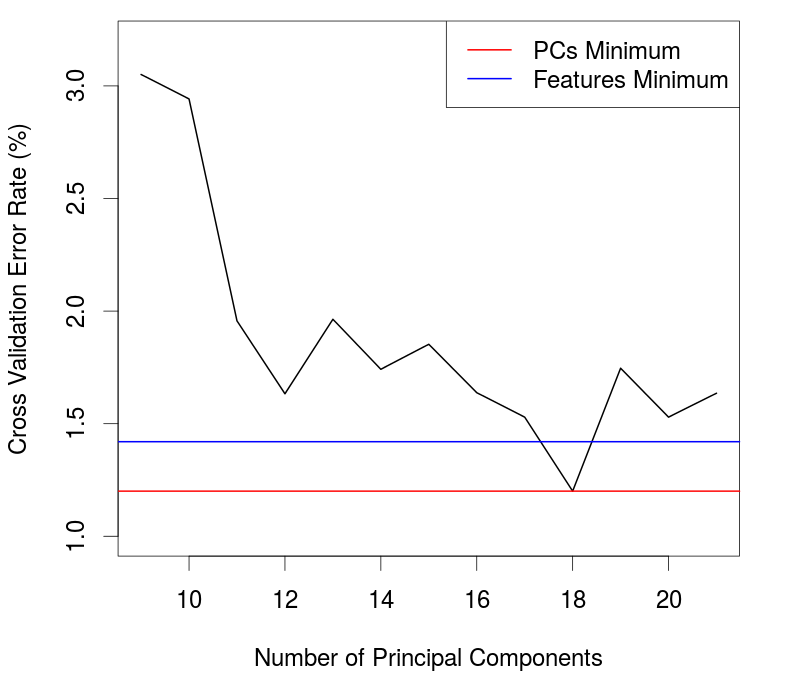
\includegraphics[width=.5\linewidth]{images/pcaEffect}
		\caption[Effect of PCA]{Effect of PCA. Black line represents error rate using a certain number of principal components. Red and blue lines show minimum error rates for fit using principal components and fit using extracted features, minimum error rates equal 1.42\% and 1.2\% respectively.}
		\label{fig:pcaEffect}
	\end{figure}
	
	Another method to do feature selection, which is used in this analysis, is to iteratively fit classifiers for any reasonable number of principal components and track error rate over fits. Figure \ref{fig:pcaEffect} shows that PCA improves not only error rate, which was decreased from 1.42\% to 1.2\%, but also removes unnecessary information since in optimal case only 18 out of 21 principal components are used. It is also reasonable to mention how fast error rate degradates at early stages. Starting from roughly a half of all components - 11 principal components, error rate is lower than 2\% that makes predictions very accurate. 
		
	\subsection{Multi Class SVM}
	Initially SVM technique was proposed as a binary classifier. However in this analysis underlaying problem requires division between six classes: three normal and three failure ones. ``One to Others'' and ``One Against One'' modifications of SVM were proposed to deal with this limitation. In ``One to Others'' method there are basically two classes in each optimization process: one class and the others as the other class. The winner is defined as class with the maximum distance to decision boundary. ``One Against One'' approach uses $k(k - 1)/2$ classifiers for $k$-class problem. Here each classifier is trained on data from two classes. After training process winner class can be deduced using voting scheme.      
		
	Instead of creating several binary classifiers, a more natural way is to distinguish
	all classes in one single optimization process.	Initially Weston and Watkins proposed $k$-class SVM \cite{weston1998multi}. Further modification was proposed by Crammer and Singer \cite{crammer2001algorithmic}. These methods generalize optimization problem of binary case for $k$-classes, however final complexity impedes extensive use of these approaches in practice.
	
	So far in this analysis ``One Against One'' approach was used. Model consisted of 15 binary SVM classifiers and winer was deduced using voting procedure: class with the highest number of votes is a winner. However other approaches should be considered as well. Since ``One to Others'' approach can bring unbalance into already balanced training data it was excluded form consideration. Table \ref{table:multiSVM} represents comparison of different approaches.  
	
	\begin{table}[h!]
		\centering
		\begin{tabular}{ | l | c | c | c | }
			\hline
			\multicolumn{1}{ | c | }{\textbf{Method}}
				& \multicolumn{1}{ | p{2.5cm} | }{\textbf{Classifiers}} 
				& \multicolumn{1}{ | p{2.5cm} | }{\centering \textbf{CV Error \\Rate (\%)}} 
				& \multicolumn{1}{ | p{2.5cm} | }{\centering \textbf{Elapsed \\Time (sec)}}\\
			\hline
			``One Against One'' & 15 	& 1.2 	& 5.2\\
			Crammer and Singer 	& 1 	& 2.28	& 6.1\\
			Weston and Watkins 	& 1 	& 29.58	& 11.2\\
			\hline
		\end{tabular}
		\caption[Multi Class SVM]{Multi Class SVM. CV Error Rate represents 20-fold cross-validation error rate on balanced training dataset.} 
		\label{table:multiSVM}
	\end{table}
	
	It can be seen from Table \ref{table:multiSVM} that multi class modifications do not benefit computational performance and final accuracy of classifier at all. Moreover error rate using Weston and Watkins multi class method is dramatically higher. It can be possibly explained by the fact of inappropriate parametrization, since default parameters were used in experiments. In addition, computational time for this method more than twice longer than time to build 15 standard binary SVM classifiers.	
	
	\subsection{Parameter Optimization}
	So far model was build under default parameters. More precisely, regularization strength parameter $C$ of SVM classifier equals 1 and ANOVA RBF kernel has a vector of parameters $\alpha=\left(\sigma=1, d=1\right)$. Of course, proper parametrization is an open problem in failure pattern recognition. It requires time and expensive computational resources, however accuracy can significantly benefit from such optimization. In area of machine fault diagnosis a variety of methods were proposed to cope with that problem: GAs, Particle Swarm Optimization (PSO) and Grid Search (GS).
	
	In this analysis in order to optimize parameters PSO proposed by Kennedy, Eberhart and Shi \cite{shi1999empirical} is used. This method is mainly based on behavior of animals then they are trying to find the source of food. Optimization experiment used 25 iterations of algorithm with default settings specified for function \textit{psoptim} of package \textit{pso}\footnote{https://cran.r-project.org/web/packages/pso/pso.pdf} built in R.       
		
	\begin{figure}[h!]
		\centering
		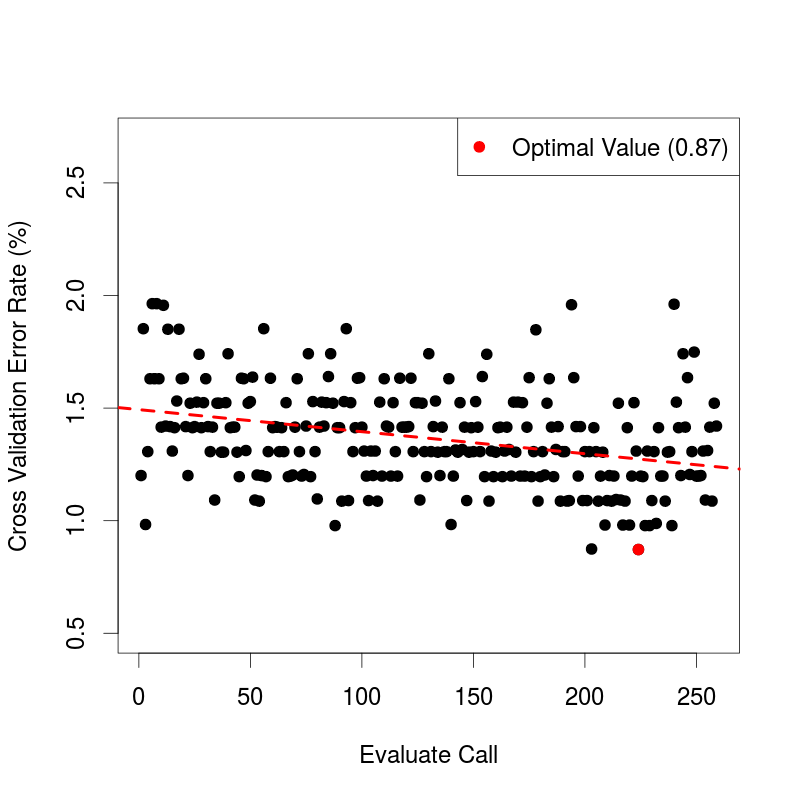
\includegraphics[width=.5\linewidth]{images/optimization}
		\caption[Parameter Optimization]{Parameter Optimization. Black points represent fitness of a single model evaluation, optimal fitness is 0.87\% of 20-fold cross validation error rate.}
		\label{fig:optimization}
	\end{figure}
	
	Figure \ref{fig:optimization} represents search procedure of optimal parameters. It can be seen that general trend is decreasing over iterations. In the end of optimization, final 20-fold	cross validation error decreased from 1.2\% to 0.87\%. The regularization strength parameter $C$ changed from 1 to 20.65 that basically means that decision margin of classifier become thinner. Parameters of kernel changed as well, initial vector $\alpha=\left(\sigma=1, d=1\right)$ moved to $\alpha'=\left(\sigma=0.77, d=1.03\right)$. However optimization process was very computationally exhaustive and took about 72.5 minutes for 25 iterations, in comparison one fit lasts only 5.5 seconds.
	
	Two remarks should be done here. First, found parameters are ``pseudo'' optimal since PSO is just a heuristic and does not provide global solutions. Second, estimated error rate is robust but can change, since division to folds in cross validation is stochastic. It can be fixed in two ways: increasing number of folds or setting up replication for evaluation of fitness. Replication means that error rate for a set of parameters will be calculated multiple times and then averaged. Both methods improve quality of optimization but increase complexity. 
	
	\subsection{Final Model and Further Modifications}
	After all improvements and modifications final model incorporates ``One Against One'' approach as well as voting scheme to extend SVM for multi class problem. Therefore 15 standard ``$C$'' implementations of SVM with parameter $C=20.65$ are build to distinguish between each pair of classes. Kernel transformation for every binary classifier is ANOVA RBF with a vector of parameters $\alpha=\left(\sigma=0.77, d=1.03\right)$. Model is fitted on first 18 principal components extracted from initial data. Training data are balanced with use of ``Smean'' technique explored in Section \ref{samplingMethods}. Final 20-fold cross validation error rate equals 0.87\% which makes model very accurate.
	
	\begin{table}[h!]
		\centering
		\begin{tabular}{ l | c | c | c | c | c | c | }
			\multicolumn{1}{ c | }{\textbf{}}
				& \multicolumn{1}{ | c | }{\textbf{Norm. 1}} 
				& \multicolumn{1}{ | c | }{\centering \textbf{Norm. 2}}
				& \multicolumn{1}{ | c | }{\centering \textbf{Norm. 3}}
				& \multicolumn{1}{ | c | }{\centering \textbf{Fail. 1}}
				& \multicolumn{1}{ | c | }{\centering \textbf{Fail. 2}} 
				& \multicolumn{1}{ | c | }{\centering \textbf{Fail. 3}}\\
			\hline
			\textbf{Norm. 1} & \textbf{229} 	& 0 			& 1				& 0 			& 0 			& 0\\
			\textbf{Norm. 2} & 0 				& \textbf{249} 	& 1				& 0 			& 0 			& 0\\
			\textbf{Norm. 3} & 0 				& 3 			& \textbf{228}	& 0 			& 0 			& 0\\
			\textbf{Fail. 1} & 0 				& 0 			& 0				& \textbf{90}	& 0 			& 0\\
			\textbf{Fail. 2} & 1 				& 0 			& 0				& 0 			&\textbf{19}	& 0\\
			\textbf{Fail. 3} & 2 				& 0 			& 0				& 0 			& 0 			& \textbf{90}\\
			\hline
		\end{tabular}
		\caption[Confusion Matrix for Final Model]{Confusion Matrix for Final Model. Norm. is short for Normal and Fail. is short for Failure respectively. Actual classes are arranged in columns, predicted classes in rows.} 
		\label{table:confusionMatrix}
	\end{table}	
	
	Table \ref{table:confusionMatrix} shows final confusion matrix obtained testing model on initial unbalanced data. Overall accuracy of predictions is 99.1\% with error rate 0.9\% which is very close to obtained earlier cross validation error rate estimation of 0.87\%. It is reasonable to mention that none of observations from failure classes were misclassified, however some observations from normal classes were recognized as failures. There is also some overlap between normal classes. These results were expected and can be explained that during balancing normal classes were undersampled and failure classes oversampled therefore model already seen all observations from failure classes and only a portion of observations from normal classes.
	
	So far provided data were aggregated in time window of 5 seconds, it basically means what the answer for a question: ``Under which conditions does system operate now?'' can be answered in 5 seconds. However in some scenarios this response time is not enough. From one side, logically decrease of response time will negatively affect accuracy, since one observation is not that informative, but from the another side it will make model more sensitive to failures. Additionally, since time window is decreasing, size of training data is increasing and computational overhead may arise. These scenarios can be explored through simulation experiments using provided data. 
	
	\begin{table}[h!]
		\centering
		\begin{tabular}{ | c | c | c | }
			\hline
			\multicolumn{1}{ | p{2.5cm} | }{\centering \textbf{Response \\Time (sec)}} 
				& \multicolumn{1}{ | p{2.5cm} | }{\centering \textbf{CV Error \\Rate (\%)}} 
				& \multicolumn{1}{ | p{2.5cm} | }{\centering \textbf{Elapsed \\Time (sec)}}\\
			\hline
			0.5 & 4.97\% 	& 184.8\\
			1 	& 1.72\% 	& 60.6\\
			3 	& 0.66\% 	& 26\\
			5 	& 0.87\% 	& 21.5\\
			10 	& 0.81\% 	& 20.2\\
			20 	& 0.34\% 	& 17.5\\
			\hline
		\end{tabular}
		\caption[Affect of Response Time]{Affect of Response Time. CV Error Rate represents 20-fold cross-validation error rate on balanced training dataset. Elapsed time represents overall time to preprocess data, balance and fit classification model using SVM.} 
		\label{table:responseTime}
	\end{table}     
	
	It can be seen from Table \ref{table:responseTime} that there is decreasing trend in error rate which was expected and matches with logic. However there is one exclusion, accuracy for response time of 3 seconds is better than for 5 or even 10 seconds. It can be explained by the fact that error rate is stochastic and true error rate for that response time should be somewhere in range between 0.87\% to 1.72\%. To summarize this comparison it can be proposed to use response time equals 1 or 3 seconds. However, further decrease hardly can be done in practice since aggregation in time window of 0.5 second significantly affect computational time and accuracy.
	
	One practical problem normally arises in area of failure pattern recognition. It is impossible to get all the failure data in advance: failures are not discovered yet or arriving very slowly as system is aimed to work without them. The straightforward way can be here is to wait for further failures and then retrain classifier incorporating arrived data. Of course, it is not advisory method in practice. Another way to cope with the problem is to use one-class SVM. This method was initially proposed by Scholkopf et al. \cite{scholkopf1999support}. The idea behind this method is to construct a representational model of normal training data. Then if newly arriving data are too different according to some measurements they labeled as out-of-class.
	
	To explore performance of one-class SVM provided data are preprocessed and aggregated in time window of 5 seconds as before. Training data consist of 80\% of observations from Normal 1 class, other normal classes were excluded as they were obtained under pressure conditions. Test data consist of the rest 20\% from Normal 1 class and all observations from failure classes. Kernel transformation is ANOVA RBF with vector of parameters $\alpha=\left(\sigma=1, d=1\right)$ 
	
	\begin{table}[h!]
		\centering
		\begin{tabular}{ l | c | c | c | c | }
			\multicolumn{1}{ c | }{\textbf{}}
				& \multicolumn{1}{ | c | }{\textbf{Normal 1}} 
				& \multicolumn{1}{ | c | }{\centering \textbf{Failure 1}}
				& \multicolumn{1}{ | c | }{\centering \textbf{Failure 2}}
				& \multicolumn{1}{ | c | }{\centering \textbf{Failure 3}}\\
			\hline
			\textbf{Normal} 	& \textbf{35} 		& 3 			& 1				& 9\\
			\textbf{Failure} 	& 12 				& \textbf{87} 	& \textbf{18}	& \textbf{81}\\
			\hline
		\end{tabular}
		\caption[Confusion Matrix for One-Class SVM]{Confusion Matrix for One-Class SVM. Actual classes are arranged in columns, predicted classes in rows.} 
		\label{table:confusionMatrixOneClassSVM}
	\end{table}	
	
	It can be seen from Table \ref{table:confusionMatrixOneClassSVM} that even without knowing actual failures one-class SVM can recognize them with high level of confidence. The final accuracy rate for that model is 89.8\%. However about 25\% of observations from class Normal 1 were misclassified, in practice it means that there will be a lot of false alarms. In spite of that fact, majority of failure observations were classified correctly which highlights applicability of one-class SVM.
	
	\section{Results and Conclusion}
	The first question that should be discussed here is feasibility of results. Final accuracy, obtained in this analysis, is extremely high and should be considered very cautiously. Good results can be explained by several reasons. First, crucial role here is purity of provided data. Data do not have outliers or missing values and can be even ``artificial'' since they were generated in test environment. Second, balancing techniques improve accuracy of predictions. Third, dimensionality reduction and feature selection as well as SVM tuning benefit results.
	
	During the analysis following fundings were explored. Removing steady states at data preprocessing stage improves further results. Aggregation of data in a certain time window is required and makes classification even possible. Also balancing mildly imbalanced data still can improve classification results. PCA slightly decreases needed amount of features and improves accuracy. This analysis shows that based on generated data ANOVA RBF transformation outperforms other kernels. Further optimization of classifier and kernel parameters can be done with help of PSO, but it is computationally expensive. Required response time can be decreased to 1 second, but it takes 3 times longer to train. From other hand, classifier, based on response time of 3 seconds, is slightly longer to build, but accuracy even better.      
	
	This analysis does not pretend to be exhaustive therefore a variety of improvements can be done in order to improve results. First, feature extraction can be extended, for example, frequency-domain features can be used to capture physical concept of a signal. This approach was explored by Soleimani et al. \cite{soleimani2009fault} and brought positive results. Second, at early stages more detailed preprocessing step can be done, for example data normalizing. Third, one can propose to apply more sophisticated $k$-class sampling methods. Fourth, more advanced dimensionality reduction techniques, such as ICA or nonlinear modifications of PCA and ICA, as well as advanced feature selection methods, for example, Distance Evaluation Techniques, can be applied. Another improvement is to try different methods of SVM, such as $\nu$-SVM or $\epsilon$-SVM, and different approaches of multi class SVM adaptations, for example``One-Against-Other'' method. One can also propose to analyze relative importance of features, in other words find small subset of untransformed features which can be used to separate classes. This can be used in order to understand the causality effects of vibration on failure states. One technique that can be applied here is Recursive Feature Elimination (RFE). RFE is aimed to get a ranked list of features. Features are sorted relatively to contribution of SVM accuracy and therefore top of them can be used to solve above task. This method was applied by Tian et al. \cite{Tian2015296} in steel plates failure pattern recognition.    	
	
	\bibliographystyle{plain}
	\bibliography{References}
	\newpage
	
	\section*{Declaration of Authorship}
	We hereby declare that, to the best of our knowledge and belief, this Seminar Thesis titled ``Application of Data Analytics in Failure Pattern Recognition'' is our own work. We confirm that each significant contribution to and quotation in this thesis that originates from the work or works of others is indicated by proper use of citation and references.
	\\\\	
	M�nster, \today
		
\end{document}